\newpage
\part{Design}

    \graphicspath{{images/design/}}


    \section{Networks}
        
        \subsection{Data in/out}

        Each model should be able to work with 4 points of data at every time unit: open, high, low, close, or less. This is to fit the structure of incoming/real-world data provided by the AlphaVantage api (FX Intraday). 

        To train/test our agents, a dataset of open/high/low/close/volume from a six year period on the EURUSD market with 15 min intervals will be used. We will start tests using an 80/20 split of training data to test data, as this is a good balance between ensuring that the agent learns enough during training and accurately assessing the agent's ability. 

        Neural networks work better when inputs are normalised i.e. take on values between -1, and 1. To achieve this (or at least a proxy for this), raw input values were changed to \textbf{\textit{(actual value - the mean of close prices of the window) * 100}} (the window is the time range for which the network is given inputs) Even for large windows, inputs to the network would very rarely exceed 1 or -1.

        For outputs the inital plan was to let the network choose from one of three options - the price at a timestep will be within the spread of, or greater/lower than the spread of the most recent timestep. Each option would have a confidence level - the percentage chance the network attributes to that outcome.

        \subsection{Proposed Networks}

        We have two problems to consider with the how inputs to the network. Firstly we need the network to be able to see many previous time steps as this is what will likely allow it to predict prices correctly if anything. Secondly, for each time step, we have 4 data points - open, high, low, close.

        A variety of input arrangements were proposed for the networks.

        \begin{itemize}

            \item \textbf{Feed-forward Networks:} All the feed-forward networks below would have a 1D convolutional layer as the first input layer, convolving each of the four inputs for a timestep (open, high, low, close) and producing one output for the next layer

            \begin{itemize}
                    
                \item \textbf{Normal deep learning network:} The network would be made up of standard feed-forward connections in which every ouput in one layer would be an input to every node in the next layer. While straightforward to implement, this requires many neurons to train 

                \item \textbf{Casually dilated convolutions:} This technique was inspired by Deepmind's wavenet \cite{wavenet}. It has the advantage of being able to look back on many previous timesteps while having a relatively small number of neurons to train. The structure of the network has the shape of a binary tree, where each layer has half the neurons of the last and each neuron takes two inputs from the previous layer. This allows the network to have a large lookback period without requiring many neurons.
            
                \item \textbf{Exponetially increasing merged timesteps:} This setup is motivated by the assumption that the further back in the past the data is, the less relevant it is. For this, we will take current set of 15 min data (0 to -15), the set of data from -15 to -30, then -30 to -60, -60 to -120, -120 to -240 and so on (if needed). To merge timesteps, we take the open value of the timestep furthest back in the past for the window we are looking at, the close from the most recent, and the maximum high value and minimum low value throughout the range. 
            
            \end{itemize}

            \item \textbf{Recurrent Networks:} Recurrent networks are good at solving problems that have a sequential nature, such as time series problems. Because of this, they are very appropriate for the problem at hand, however they take longer to train \cite{wavenet}.
            
            \begin{itemize}

                \item \textbf{LSTMs}: LSTM (Long-Term Short Memory) networks are especially good at solving sequenced problems as each lstm unit in the network chooses to remember of forget certain values depending on how important the network deems the value to be.
                
            \end{itemize}

        \end{itemize}

        It was decided that a feed-forward network with "normal inputs" and a recurrent network should be tested before the other feed-forward networks as they would be more difficult to implement


        \subsection{Training Process}

            \subsubsection{First Network}
            The initial model was a normal deep learning network. N previous sets of OHLC data were fed to the network and 3 outputs were given, representing the probability the network gave to the price moving up, down and staying within the typical spread price.

            As discussed above, the first layer was a 1D convolution that created one output for each set of OHLC data. For the other hidden layers, a number of setups were tested, with usually a starting layer of 64 neurons. The output layer had three neurons with a softmax \footnote{A softmax is a function that normalises a number of values. This is often used to get probabilities from an output layer.} applied so the network outputs represented the probability the network assigned to the price moving up, down, or staying within the spread. The network was initially setup with the SGD optimiser, with a small learning rate of 0.01 as is customary for deep supervised learning.
            
            \begin{figure}[h]
                \centering
                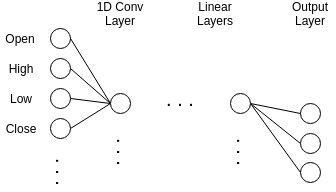
\includegraphics[width=0.8\textwidth]{Conv-Net.png}
                \caption{Network Diagram}
                \label{fig:first_net_diagram}
            \end{figure}

            As a preliminary test, it was decided the network should try to overfit \footnote{Overfitting is where a network learns the test data and corresponding outputs it is given instead of being able to generalise and learn which features of the inputs cause certain outputs, thus performing very badly on unseen data. This usually happens when the size of the test data is too small} on a small batch first. The network greatly struggled with this however. On every run the network would either converge on a solution that assigns equal probability to each outcome, or one that always assigns 100\% to the price increasing or decreasing.

            Eventually, using the “Adam” optimiser instead of SGD, the network managed to overfit on the small batch of 20.\footnote{In figure ~\ref{fig:Overfit} the rows above show the output tensors from the network for the last few inputs. Below the expected outputs vs. the network ouput with the largest value (the network prediction)}

            \begin{figure}[h]
                \centering
                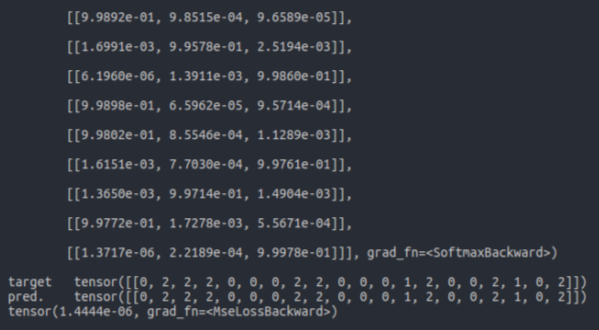
\includegraphics[width=0.8\textwidth]{overfit.png}
                \caption{Output from running the overfitting test.}
                \label{fig:Overfit}
            \end{figure}
            

            It was thought that the reason Adam worked was because the problem is quite complex and thus SGD (steepest gradient descent - which takes steps only in the direction of the steepest gradient) was less likely to have found the global minimum of the cost function, whereas Adam, which is stochastic, is better at “exploring” the landscape of the cost function and so more likely to find the global minimum.

            When attempting the actual training (using the entire training dataset), all runs gave unsatisfactory results. At best networks gave the correct prediction around 49\% of the time. Given that at the 15 minute interval the price moves up/down around 45\% of the time and stays within the spread the remaining 10\%, the network was not giving desirable predictions (the network was barely doing better than random guesses).

            The approach that was taken to this problem of mapping the inputs onto one of three discrete outputs was influenced by classic classification problems such as recognising images of handwritten digits in which there is a clear "correct" mapping between the inputs onto one output. However forex prices are stochastic - it is possible to determine with certainty given a set up of inputs what the "correct" output should be so it was thought that training a network using the three discrete outputs (price up, down, same) represented as a [1, 0, 0], was causing problems during optimisation.

            It was decided that a network with a different structure should be tested.


            \subsubsection{LSTM Network}
            It was decided that the next test should be an LSTM network that predicted the price itself. N individual sets of OHLC values would be fed one by one into the network with one LSTM layer and one single output neuron. The Adam optimiser was used with learning rates from 0.05-0.4.

            \begin{figure}[h]
                \centering
                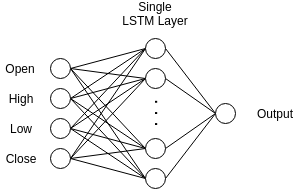
\includegraphics[width=0.8\textwidth]{LSTM-Net.png}
                \caption{Network Diagram}
                \label{fig:LSTM_Diagram}
            \end{figure}

            The network produced what were thought to be far more desirable results, with initial tests able to predict the price in 15 mins correctly within the spread (taken as 0.7 pips) roughly 60\% of the time . This was initially surprising as originally, it was initially thought that predicting the price itself was a more difficult problem than just predicting the discrete movement of the price.

            //predictions here

            The concern was that the network seemed to be just quoting the most recent close price at each (see **).


            There were a few suggestions about why this might have been the case and how to improve on it.

            \begin{itemize}
                \item \textbf{Too few neurons} The network was not large enough and so couldn't learn the more complex behaviours required.
                
                \item \textbf{Window size was too large} Too much data was being fed to the network. With so many inputs it was difficult for the network to converge on a valid solution other than quoting the latest close price. Additionally, network outputs were given as movements from the mean of the window so the larger the window, the larger the window, the greater the variance of the mean in relation to the final close price, which could be affecting the validity of the predictions. 
                
                \item \textbf{Prediction time-scale too small given the data} The tests were first being done on 15 and 30 minute predictions. Given the data being fed to the network was in 15 minute intervals, it was thought that these predictions could have been too close in the future for the network to converge on effective solutions as the price would not have moved too far/any movements had too much associated noise. It was thought that over longer time-scales general trends would be able to be found and thus more effective predictions could be made.
            
            \end{itemize}
            

            It was found that adding more neurons could often result in a worse solution, likely because the network was too complex and the number of training iterations was too small to be able to properly explore the landscape of the fitness function. When decreasing the window size, it was found that the network could converge on smaller losses, and when doing tests on the predictions further in the future, returned values were thought to be better.

            \begin{figure}[h]
                \centering
                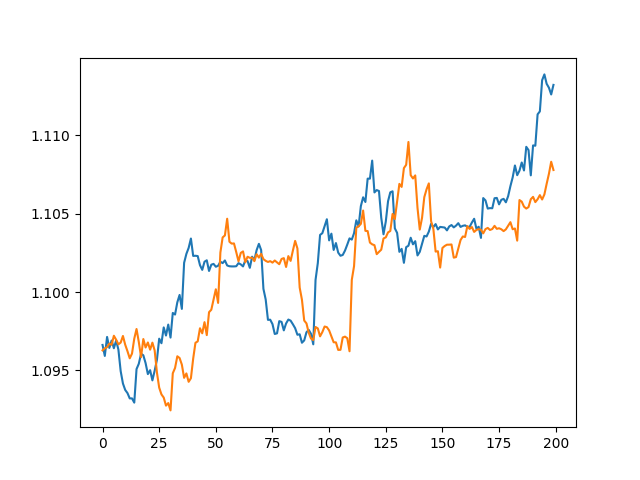
\includegraphics[width=0.8\textwidth]{240-50-30-1.png}
                \caption{Sample prices against the prediction made that timestep 4 hours (16 timesteps) beforehand}
                \label{fig:240_predictions}
            \end{figure}

            In figure ~\ref{fig:240_predictions} while it does seem that the network mostly seems to be quoting the most recent close price, at many points we can see that it is both over and undershooting peaks and troughs - showing that it is observing trends and making decisions based on data from more than just the last timestep.

            It was decided that this structure should be used in the final solution.


        \subsection{Measuring Success}

        Now it had been decided that a raw price prediction network would be used, the ability of a network was measured by two criteria - the mean squared error between the predictions and the target values, and the percentage of predictions made that fell within the high and low prices of the relevant timestep.

        As discussed above, it seemed as though the network could have been just quoting the most recent close price as the prediction. To test this - ensure the network was making "valid" predictions, a baseline was created by finding the MSE and percentage accuracy of a solution quotes the most recent close price as the prediction for a future timestep. 


        \subsection{Final networks}

        Using the above critera, the networks that were chosen to be used had the following results
        \textbf{*yeet a table of the successes in*}
        
`'
    \section{User Interface}

        \subsection{Layout}
        The predictions should be shown in a concise way graphically so that users viewing predictions via the webpage can more easily interpret the data. All data should be shown on one page.
        
        It was thought that previous market data, predictions as well as some measure of the precision of the predictions such as standard deviation of error should be displayed on one graph. If possible users should be able to choose how much data is being displayed at one time using sliders. Aon the same page, there should be a chart displaying the recent accuracy of predictions (how often the network correctly predicts the price within the actual high and low of the timestep). 

        On the page the current UTC time and the time of the data being shown should be displayed.



    \section{API}
        
        \subsection{Data Returned}
        When an API call is made, the server will check if the API key used is valid (is in the list of API keys being used). If it is, then data will be returned, else an error message will be returned.

        Data returned should be in JSON format and include all data that is shown on the webpage in numerical form. JSON was chosen as it is relatively compact, well supported and also allows for more logical represetation and ordering of data with the use of hierarchy. 

        A request should not be served if requests from the user are being made too frequently.
    

        \subsection{Signing Up}
        On the webpage, there should be a text field where a user can enter there email to get an API key. If the email is valid, a random API key will be generated and sent to the user. If the email is invalid an error message should appear. If the email has already been used to sign up, the API key should be shown.

        \subsection{Email Hashing}
        It is thought that the users would never need to be directly contacted and thus the user emails should never be stored or sent in plaintext to ensure user privacy. Were emails sent in plaintext, a "man in the middle" would be able to see the email.

        To ensure this when a user signs up for the service, their email should be hashed on the client side using MD5 with a random salt before being sent to the server. The user will then be shown their API key on the webpage.
    

        
    \section{Backend}

        \subsection{Dataflow}
        There should only be one copy of historic data and predictions to ensure data is consistent in all places and updating these is easier. Because of this, the same datafile that can be accessed via the API should be used as the source of data for the webpage.
            
            \subsubsection{Updating data}
            Every 15 minutes, the server should check for new data from AlphaVantage. Data from the API does not update every 15 minutes on the dot however so the server should keep making API calls until the time of the data changes. AlphaVantage stops fufilling requests if they exceed more than 5 requests a minute or more than 500 requests a day. Given that new data for each 15 minute timestep seemed to come roughly 5 minutes late, a 45 second delay between requests was thought to be appropriate.

            \subsubsection{Feeding data to networks}
            
            
            
        
        \subsection{Database}
        The database should be made up of a User table, storing the a hashed email and api key, and a Predictions table, storing the time of the prediction and the value of each prediction. These tables have a many to many relationship and so need a helper table.
        
        Tables required 
        \begin{itemize}

            \item \textbf{User:} Stores Email hash, API key, Date of signing up. 

            \item \textbf{Predictions:} Stores the time the prediction corresponds to and each prediction.
            
            \item \textbf{Requests:} Stores User ID, Prediction Time, current time. A helper table for the many to many relationship between the User and Predictions table. Every time a user makes an API request, an entry should be made for this table. This will allow for policing of users making requests too frequently. It will also allow for metrics such as when in the day requests are most frequently made to be calculated. 

        \end{itemize}
        
            